\chapter{Introdução}


Numa organização de desenvolvimento de software, normalmente encontra-se problema relacionado ao cumprimento dos prazos de entrega. Tal situação pode ocorrer devido a diversos fatores, a exemplo do aumento de demandas extras, desvios nos requisitos e problemas internos na equipe. Assim, a solução para atrasos de entrega pode estar em diversos fatores, entretanto, existem elementos universais que podem colaborar para a melhoria, como o reuso de software. Assim, este trabalho de conclusão de curso busca padronizar a parte de controle de acesso dos softwares, tornando-a universal para tornar possível que seja reutilizada como um serviço em qualquer circunstância de desenvolvimento, gerando assim uma redução no tempo de desenvolvimento e manutenção.


\section{Motivação}


Otimizar o desenvolvimento de um software é uma tarefa árdua e bastante estudada. A área de Engenharia de software estuda maneiras de melhorar o desenvolvimento de software através de bons processos e práticas de desenvolvimento. Qualquer melhoria durante a construção de um sistema, normalmente acaba por prover uma economia no orçamento de desenvolvimento e/ou manutenção. Assim, é possível inferir que melhorias no processo de desenvolvimento de sistemas, pode agradar desde programador, com um trabalho facilitado, até o cliente final com redução de custo.


\section{Problema} %começar de forma mais genérica


A repetição de código durante o desenvolvimento de um software, acaba por aumentar a sua complexidade e tempo de desenvolvimento. O impacto dessa má prática atinge fortemente a manutenibilidade do software, gerando grande transtorno diante de uma alteração que poderia ser simples caso estivesse bem projetado desde o começo. Assim, o reuso de código sempre é buscado num projeto. A abordagem do reuso pode inclusive, abranger mais de um projeto numa organização, fazendo que até mesmo módulos inteiros sejam reaproveitados. 


\section{Objetivos}


\begin{itemize}
	\item Objetivo geral: Seguindo a boa prática de projetar o software, o objetivo geral deste trabalho é prover o reuso de código, utilizando padões que mantenham o componente de código na melhor forma possível para ser acoplado em outros softwares sem transtorno.
	\item Objetivo específico: Reutilizar o módulo de controle de acesso de um sistema, já que o mesmo está presente sem desvios significativos nos sistemas de uma organização. Assim, o objetivo é desenvolver tal módulo como um serviço, deixando-o isolado e gerando a possibilidade de qualquer sistema consumir tal módulo como um serviço. Dessa forma, ao projetar um novo software para uma organização por exemplo, ao invés de incluir o módulo de controle de acesso, projetaria-se o código para consumir o serviço de contrle de acesso que seria um projeto à parte. Tal situação também tem a vantagem de ter interoperabilidade entre linguagens de programação, já que realizaria a comunicação através de JSON, seguindo padrões atuais. Assim, teria-se uma constância no módulo de acesso independentemente da possível necessidade de migração de tecnologia.
\end{itemize}


\section{Metodologia} %<como será feito | como resolver o problema apontado inicialmente>


%<analise de literatura | design | implementação | validação>
Baseando-se nas tecnologias gratuitas em alta no cenário atual do desenvolvimento web, dispomos de algumas opções eficientes para a implementação da solução. Dentre as possibilidades, considerando a facilidade para futura manutenção e continuidade do projeto, tende-se a optar por uma tecnologia popular. Como linguagem de programação, adota-se o PHP. A escolha é fundamentada de acordo com a pesquisa da RedMonk de 2015 \cite{Grafico-RedMonk} , que evidencia o uso das linguagens de programação de acordo com as discussões no StackOverflow e repositórios no GitHub. É possível constatar a popularidade do PHP no cenário atual com o gráfico da pesquisa citada, na qual o PHP é apresentado na terceira colocação, apenas atrás do lider JavaScript e do segundo colocado, o Java.


\begin{figure}
	\label{fig:graficoRedmonk}
	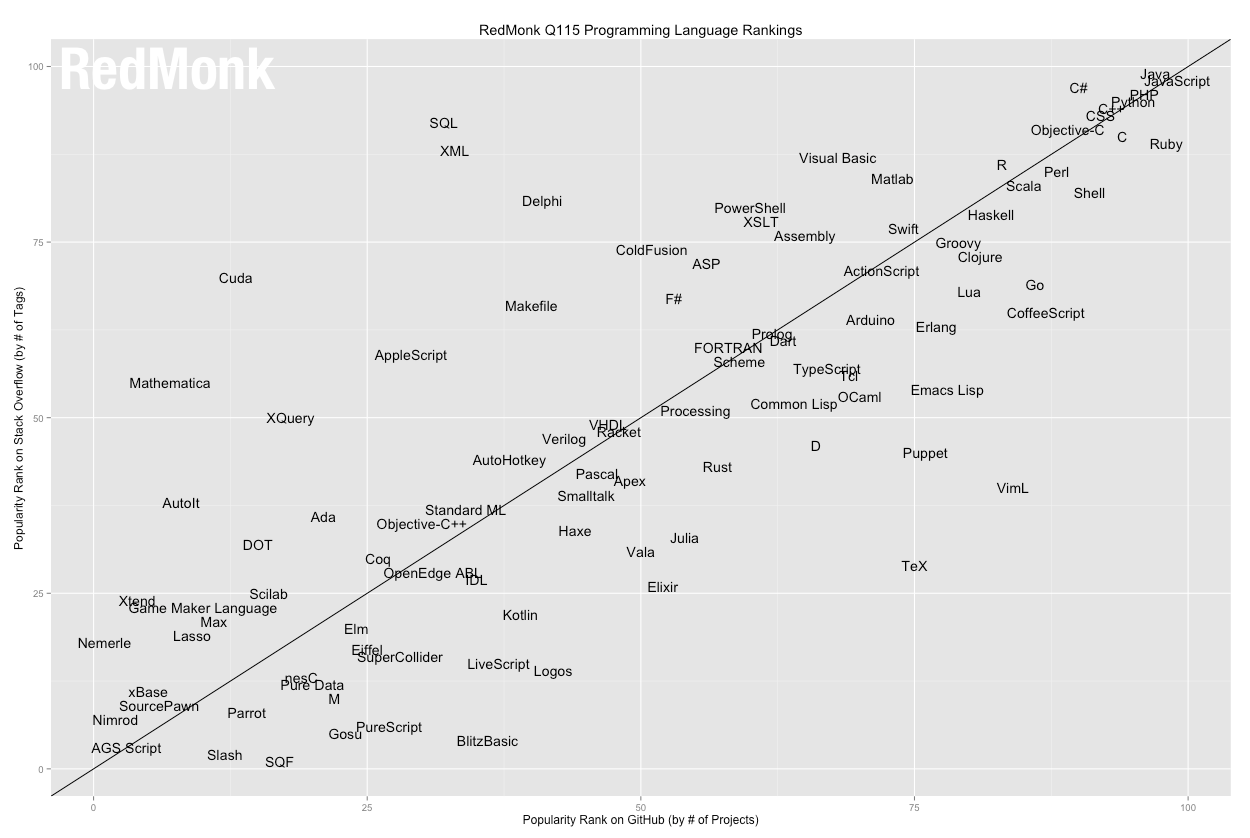
\includegraphics[width=1\textwidth]{img/grafico_redmonk}
	\caption{Ranking das liguagens de programação no Stack Overflow e Github}
\end{figure}


Entretanto, não seria inteligente desenvolver um sistema completo sem o auxílio de um framework. Dentre os frameworks disponíveis para PHP, hoje o destaque está com o Laravel, que se encontra no topo dentre os mais utilizados no momento. 
 

A WebHostFace, uma empresa de hospedagem, compilou várias estatísticas para criar um infográfico mostrando os frameworks PHP mais populares de 2015. Utilizando informações sobre os próprios clientes, o Google Trends, estatísticas de repositórios do GitHub e a pesquisa do SitePoint “Best PHP Frameworks 2015”, a WebHostFace elaborou o seguinte infográfico: %O gráfico está sendo mostrado no local errado apesar da ordem


\begin{figure}
	\label{fig:graficoWebhostface}
	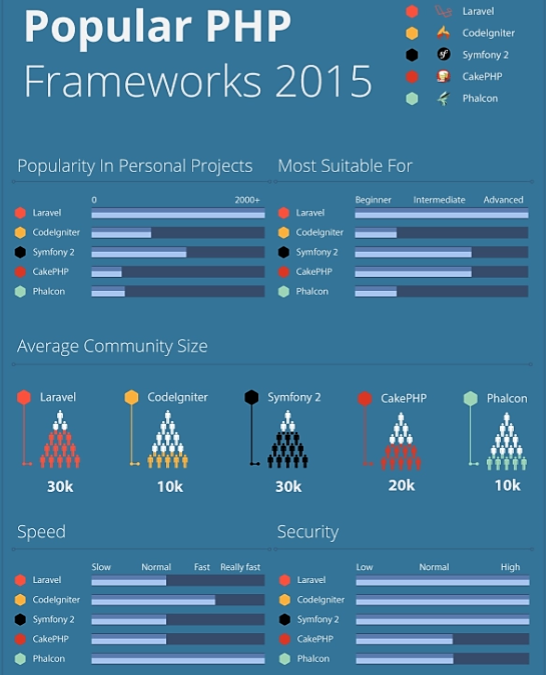
\includegraphics[width=1\textwidth]{img/infografico_webhostface}
	\caption{Infográfico da WebhostFace, exibindo a popularidade dos Frameworks PHP em 2015}
\end{figure}


Como pode ser verificado no gráfico \cite{WebhostFace-PHP-Frameworks}, tem-se a evidência que o Laravel em 2015 teve a maior popularidade em projetos pessoais e tem a maior comunidade entre os concorrentes, o que o torna uma boa escolha para a escrita de um software que será continuado por terceiros.


Para elaborar os recursos de interface e integrar ao back-end PHP do sistema, será adotado o já conhecido AngularJS, ferramenta sólida e conhecida no aspecto em questão. 


Dados coletados via Google Trends em \citealp{GoogleTrends-Front-end-Frameworks}, que propõe comparações entre termos pesquisados, revela a popularidade do AngularJs diante de alguns dos principais concorrentes. O gráfico abaixo evidencia o cenário.


\begin{figure} %Como mostra a Figura \ref{fig:graficoGoogleTrendsFerramentasFront}. 
	\label{fig:graficoGoogleTrendsFerramentasFront}
	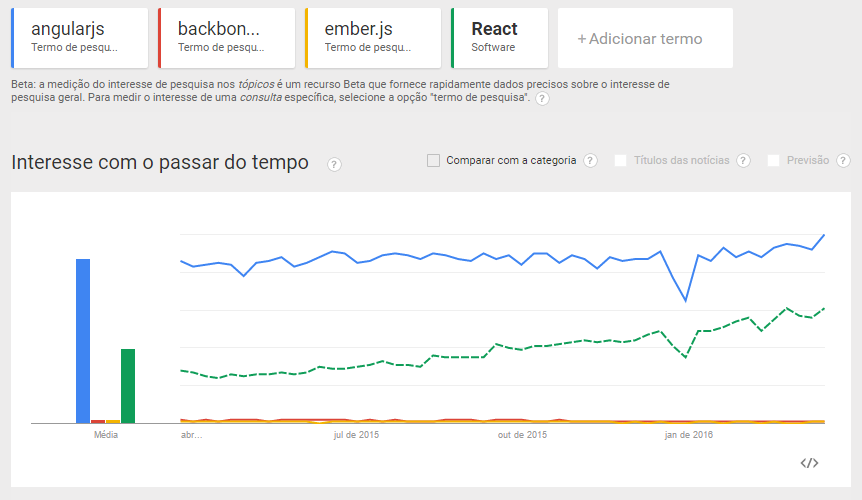
\includegraphics[width=1\textwidth]{img/grafico_ferramentas_front}
	\caption{Gráfico do Google Trends exibindo as pesquisas por ferramentas front-end}
\end{figure}


\section{Resultados Esperados}


Realizando o uso do proposto módulo de controle de acesso como serviço, espera-se que ocorram os seguintes ganhos:


\begin{itemize}
	\item Economia no tempo de desenvolvimento
	\item Economia do custo do projeto
	\item Redução da complexidade de código
	\item Maior facilidade para manutenção
\end{itemize}


\section{Fora de Escopo}


Diante da possibilidade de gerência dos sistemas, módulos e funcionalidades contratadas, seria possível estender o sistema aqui proposto, complementando-o com uma abordagem financeira, controlando o acesso do cliente mediante o pagamento do que está contratado pelo cliente. Também existe a possibilidade de realizar o controle por número de usuários que estão logados no sistema contratado ou por módulo, mediante uma evolução na implementação. Uma possível solução para a última situação seria o sistema consumidor enviar uma notificação(post) ao sistema de gerenciamento de módulo num determinado intervalo de tempo, fazendo a sinalização de que o usuário está logado no sistema. O sistema de gerenciamento de módulos responderia internamente à sinalização, mantendo registro de usuário ativo. Caso o usuário final saia do sistema, enviaria o sinal de logout e caso fechasse o navegador, a sessão seria encerrada por tempo de inatividade (falta de envio da notificação de uso).


\section{Estrutura do Trabalho} %<breve resumo sobre os capítulos do TCC>


Neste tópico, tem-se uma breve apresentação dos capítulos que compõem este trabalho de conclusão de curso:

\begin{itemize}
	\item Capítulo 1: Referencial teórico, fundamentando os principais conceitos que compõem os elementos marcantes do trabalho.
	\item Capítulo 2: Introdução, apresentando uma visão geral do trabalho.
	\item Capítulo 3: Proposta, contendo o detalhamento do trabalho proposto, baseando-se nos aterfatos da engenharia de software.
	\item Capítulo 4:
	\item Capítulo 5:
\end{itemize}

